\documentclass{article}
\usepackage[letterpaper,left=0.75in, right=0.75in, top=0.75in, bottom=0.75in]{geometry}
\usepackage{graphicx}
\usepackage[justification=centering]{subcaption}
\captionsetup[subfigure]{format=hang,justification=raggedright,singlelinecheck=false}
\usepackage{amsmath,amsthm,amsfonts,amssymb,mathtools}
\usepackage[mmddyyyy,HHmmss]{datetime}
\graphicspath{{/home/jklimavicz/Documents/merlin_stats_out/images/pdf}}
\setcounter{topnumber}{8}
\setcounter{bottomnumber}{8}
\setcounter{totalnumber}{8}
\usepackage{fancyhdr}
\pagestyle{fancy}
\fancyhf{}
\fancyhead[L]{Merlin Bioassay Results}
\fancyfoot[C]{\thepage}
\fancyhead[R]{Compiled on \today\ at \currenttime}
\renewcommand{\headrulewidth}{0pt}



%%%%%%%%%%%%%%%%%%%%%%%%%%%%%%%%%%%%%%%%%%%%%%%%%%%%%%%%%%%%%%%%\title{Merlin Bioassay Results}
\author{James Klimavicz}
\date{\today}
\begin{document}


\begin{figure}[thp!]
   \begin{subfigure}{0.500\textwidth}
      \centering
      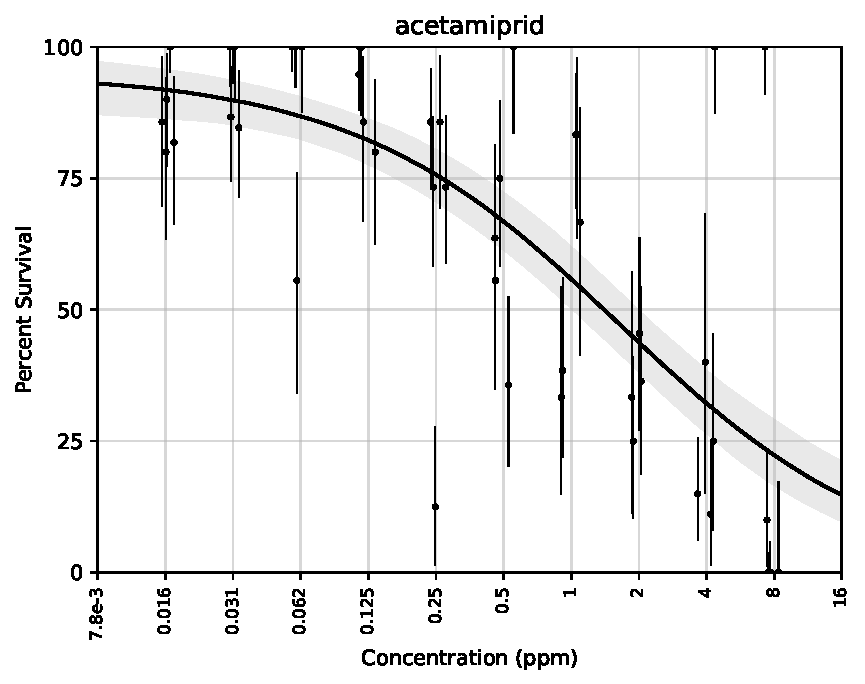
\includegraphics[width = {0.95\textwidth}]{/home/jklimavicz/Documents/merlin_stats_out/images/pdf/acetamiprid.pdf}
      \vspace{-0.05cm}
      \caption*{\textbf{Acetamiprid} LC$_{50}$: 1.61 ppm [1.06, 2.46] \\ 
4 biol. reps; 5 tech. reps; R$^2$: 0.533}
      \vspace{0.1cm}
   \end{subfigure}%
   \begin{subfigure}{0.500\textwidth}
      \centering
      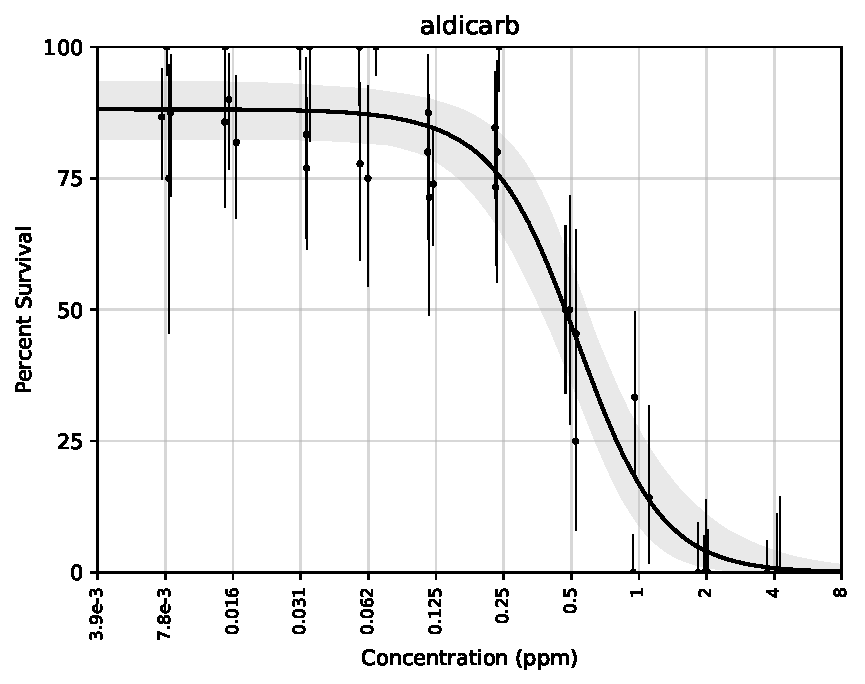
\includegraphics[width = {0.95\textwidth}]{/home/jklimavicz/Documents/merlin_stats_out/images/pdf/aldicarb.pdf}
      \vspace{-0.05cm}
      \caption*{\textbf{Aldicarb} LC$_{50}$: 0.531 ppm [0.419, 0.669] \\ 
3 biol. reps; 4 tech. reps; R$^2$: 0.935}
      \vspace{0.1cm}
   \end{subfigure}%
\vspace{-0.1cm}
   \begin{subfigure}{0.500\textwidth}
      \centering
      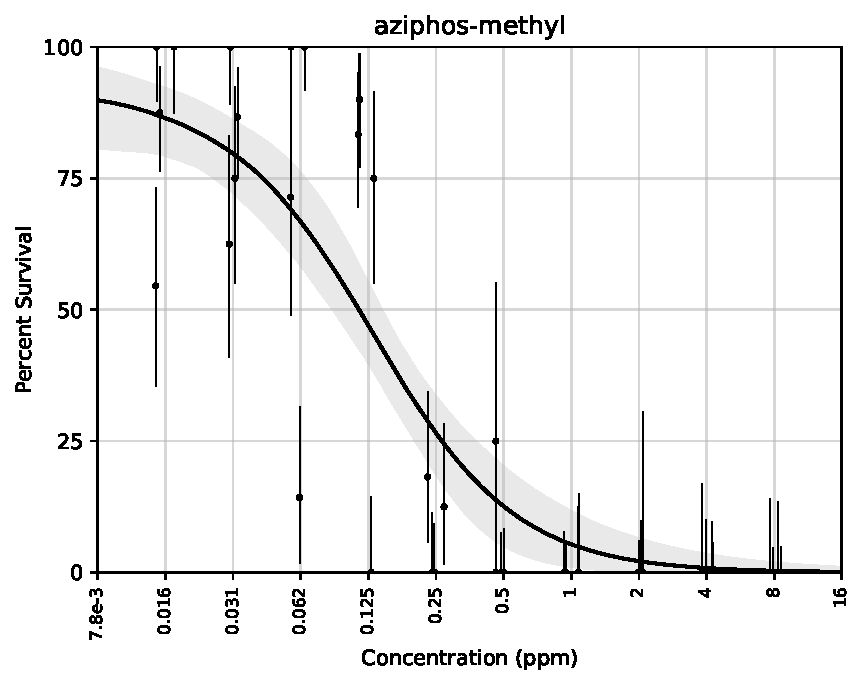
\includegraphics[width = {0.95\textwidth}]{/home/jklimavicz/Documents/merlin_stats_out/images/pdf/aziphos-methyl.pdf}
      \vspace{-0.05cm}
      \caption*{\textbf{Aziphos-methyl} LC$_{50}$: 0.128 ppm [0.0915, 0.174] \\ 
3 biol. reps; 4 tech. reps; R$^2$: 0.759}
      \vspace{0.1cm}
   \end{subfigure}%
   \begin{subfigure}{0.500\textwidth}
      \centering
      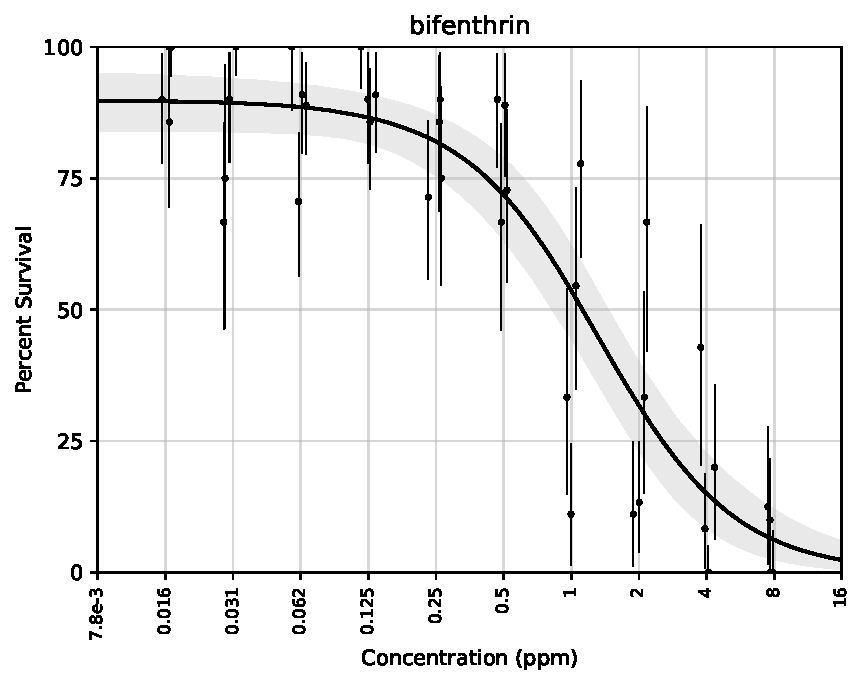
\includegraphics[width = {0.95\textwidth}]{/home/jklimavicz/Documents/merlin_stats_out/images/pdf/bifenthrin.pdf}
      \vspace{-0.05cm}
      \caption*{\textbf{Bifenthrin} LC$_{50}$: 1.31 ppm [0.965, 1.75] \\ 
3 biol. reps; 4 tech. reps; R$^2$: 0.82}
      \vspace{0.1cm}
   \end{subfigure}%
\vspace{-0.1cm}
   \begin{subfigure}{0.500\textwidth}
      \centering
      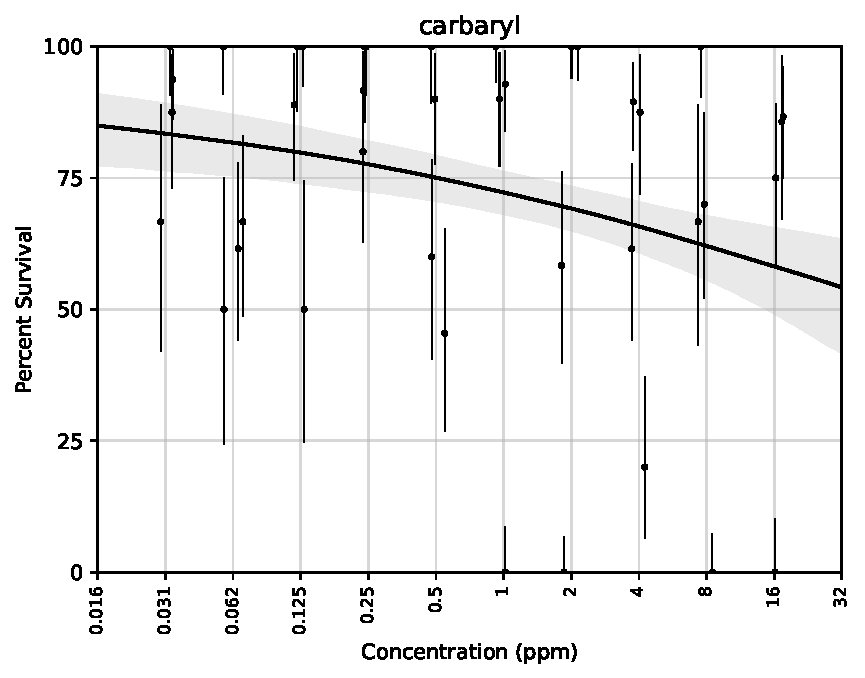
\includegraphics[width = {0.95\textwidth}]{/home/jklimavicz/Documents/merlin_stats_out/images/pdf/carbaryl.pdf}
      \vspace{-0.05cm}
      \caption*{\textbf{Carbaryl} LC$_{50}$: 88.2 ppm [14, 1.58e3] \\ 
3 biol. reps; 4 tech. reps; R$^2$: 0.0778}
      \vspace{0.1cm}
   \end{subfigure}%
   \begin{subfigure}{0.500\textwidth}
      \centering
      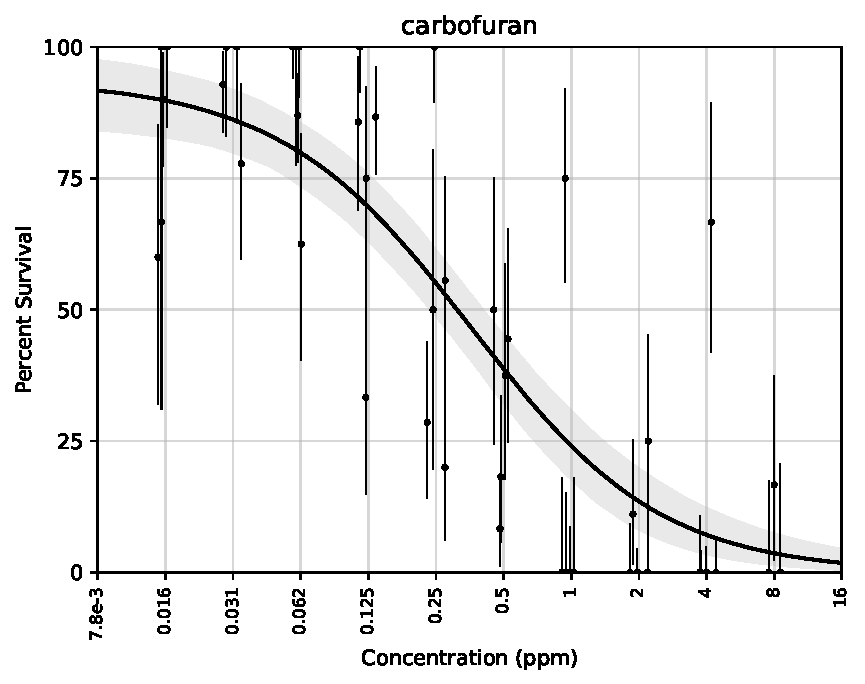
\includegraphics[width = {0.95\textwidth}]{/home/jklimavicz/Documents/merlin_stats_out/images/pdf/carbofuran.pdf}
      \vspace{-0.05cm}
      \caption*{\textbf{Carbofuran} LC$_{50}$: 0.354 ppm [0.258, 0.497] \\ 
4 biol. reps; 5 tech. reps; R$^2$: 0.728}
      \vspace{0.1cm}
   \end{subfigure}%
\end{figure}
\clearpage
\pagebreak
\vspace{-0.1cm}
\begin{figure}[thp!]
   \begin{subfigure}{0.500\textwidth}
      \centering
      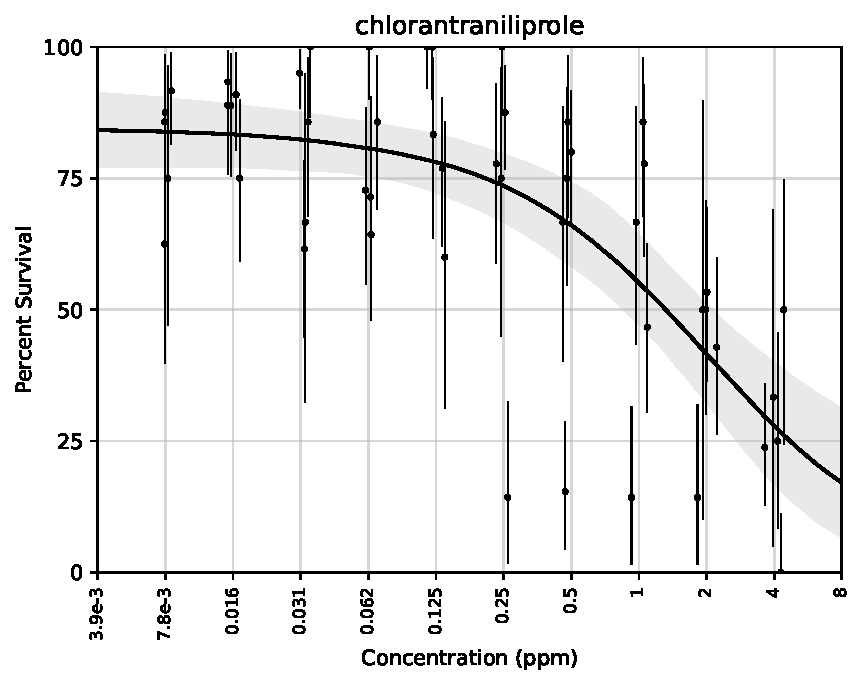
\includegraphics[width = {0.95\textwidth}]{/home/jklimavicz/Documents/merlin_stats_out/images/pdf/chlorantraniliprole.pdf}
      \vspace{-0.05cm}
      \caption*{\textbf{Chlorantraniliprole} LC$_{50}$: 1.92 ppm [1.17, 3.34] \\ 
4 biol. reps; 5 tech. reps; R$^2$: 0.501}
      \vspace{0.1cm}
   \end{subfigure}%
   \begin{subfigure}{0.500\textwidth}
      \centering
      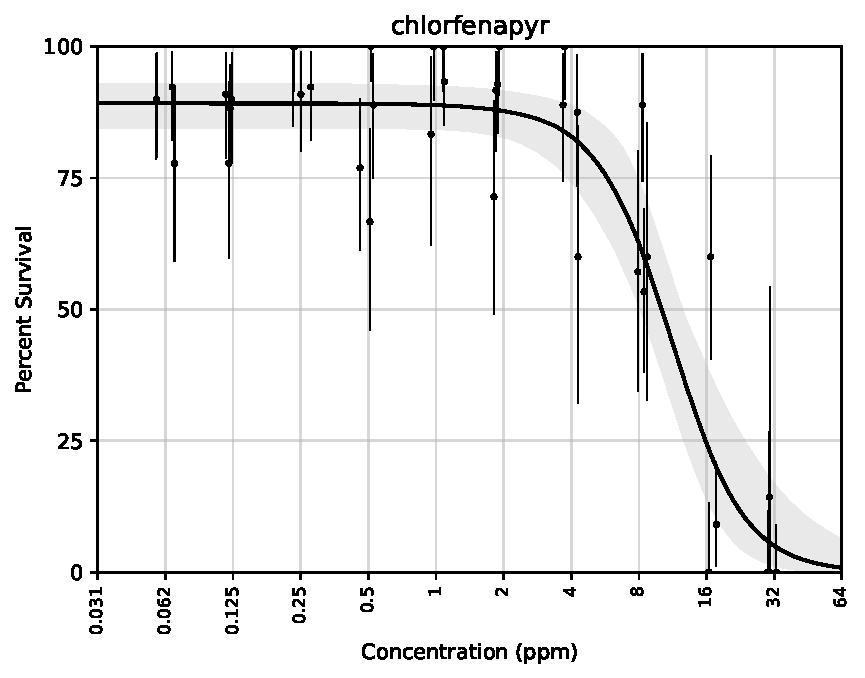
\includegraphics[width = {0.95\textwidth}]{/home/jklimavicz/Documents/merlin_stats_out/images/pdf/chlorfenapyr.pdf}
      \vspace{-0.05cm}
      \caption*{\textbf{Chlorfenapyr} LC$_{50}$: 11.1 ppm [8.93, 13.9] \\ 
3 biol. reps; 4 tech. reps; R$^2$: 0.853}
      \vspace{0.1cm}
   \end{subfigure}%
\vspace{-0.1cm}
   \begin{subfigure}{0.500\textwidth}
      \centering
      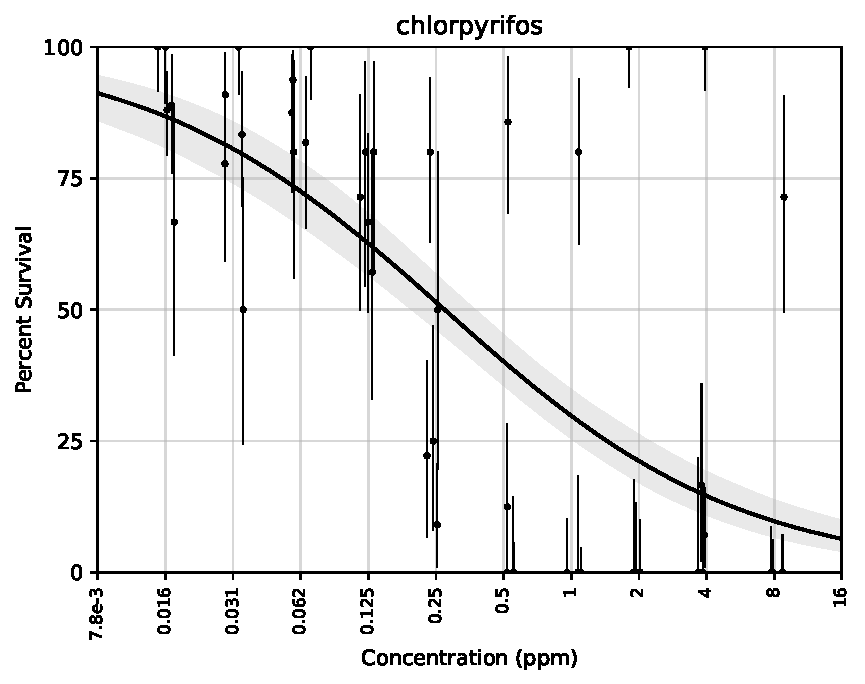
\includegraphics[width = {0.95\textwidth}]{/home/jklimavicz/Documents/merlin_stats_out/images/pdf/chlorpyrifos.pdf}
      \vspace{-0.05cm}
      \caption*{\textbf{Chlorpyrifos} LC$_{50}$: 0.274 ppm [0.199, 0.375] \\ 
4 biol. reps; 5 tech. reps; R$^2$: 0.485}
      \vspace{0.1cm}
   \end{subfigure}%
   \begin{subfigure}{0.500\textwidth}
      \centering
      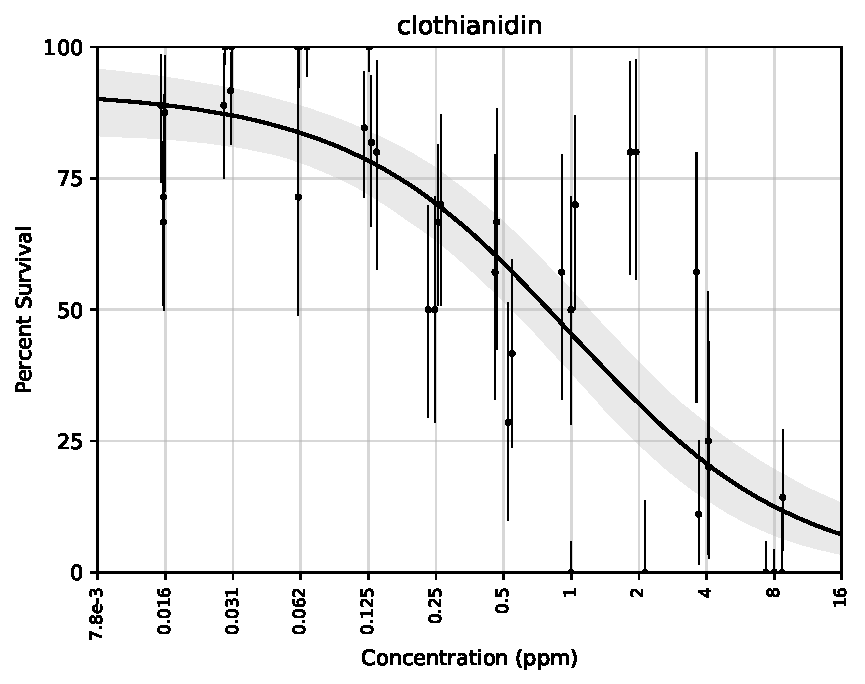
\includegraphics[width = {0.95\textwidth}]{/home/jklimavicz/Documents/merlin_stats_out/images/pdf/clothianidin.pdf}
      \vspace{-0.05cm}
      \caption*{\textbf{Clothianidin} LC$_{50}$: 0.983 ppm [0.614, 1.59] \\ 
3 biol. reps; 4 tech. reps; R$^2$: 0.651}
      \vspace{0.1cm}
   \end{subfigure}%
\vspace{-0.1cm}
   \begin{subfigure}{0.500\textwidth}
      \centering
      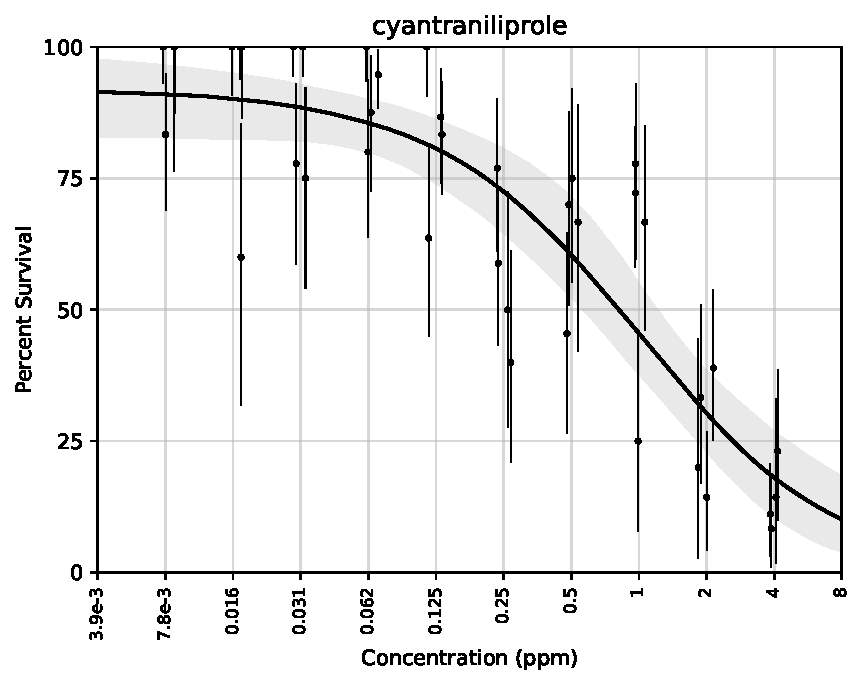
\includegraphics[width = {0.95\textwidth}]{/home/jklimavicz/Documents/merlin_stats_out/images/pdf/cyantraniliprole.pdf}
      \vspace{-0.05cm}
      \caption*{\textbf{Cyantraniliprole} LC$_{50}$: 0.974 ppm [0.616, 1.54] \\ 
3 biol. reps; 4 tech. reps; R$^2$: 0.753}
      \vspace{0.1cm}
   \end{subfigure}%
   \begin{subfigure}{0.500\textwidth}
      \centering
      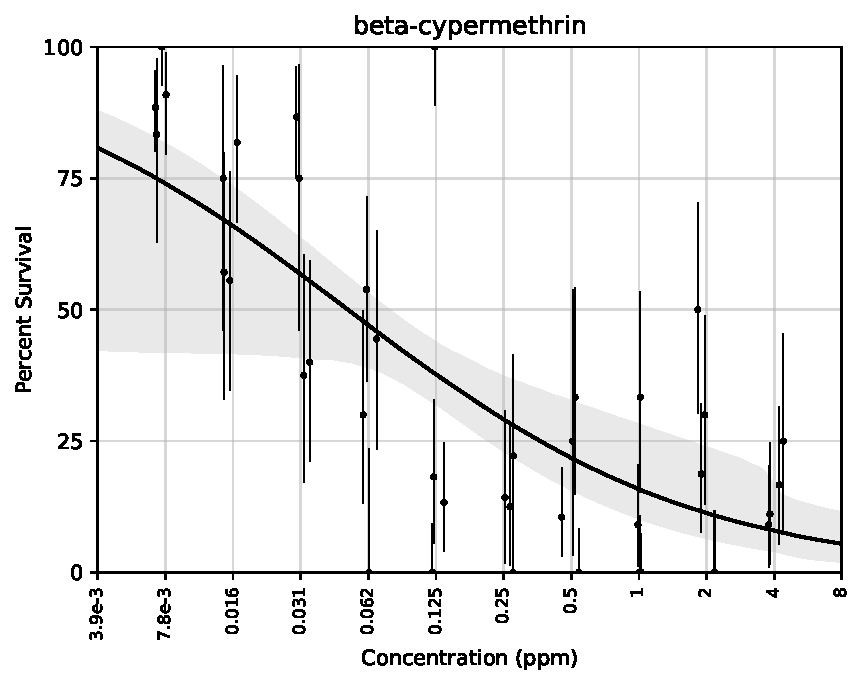
\includegraphics[width = {0.95\textwidth}]{/home/jklimavicz/Documents/merlin_stats_out/images/pdf/beta-cypermethrin.pdf}
      \vspace{-0.05cm}
      \caption*{\textbf{$\beta$-Cypermethrin} LC$_{50}$: 0.0523 ppm [0.0216, 0.111] \\ 
3 biol. reps; 4 tech. reps; R$^2$: 0.555}
      \vspace{0.1cm}
   \end{subfigure}%
\end{figure}
\clearpage
\pagebreak
\vspace{-0.1cm}
\begin{figure}[thp!]
   \begin{subfigure}{0.500\textwidth}
      \centering
      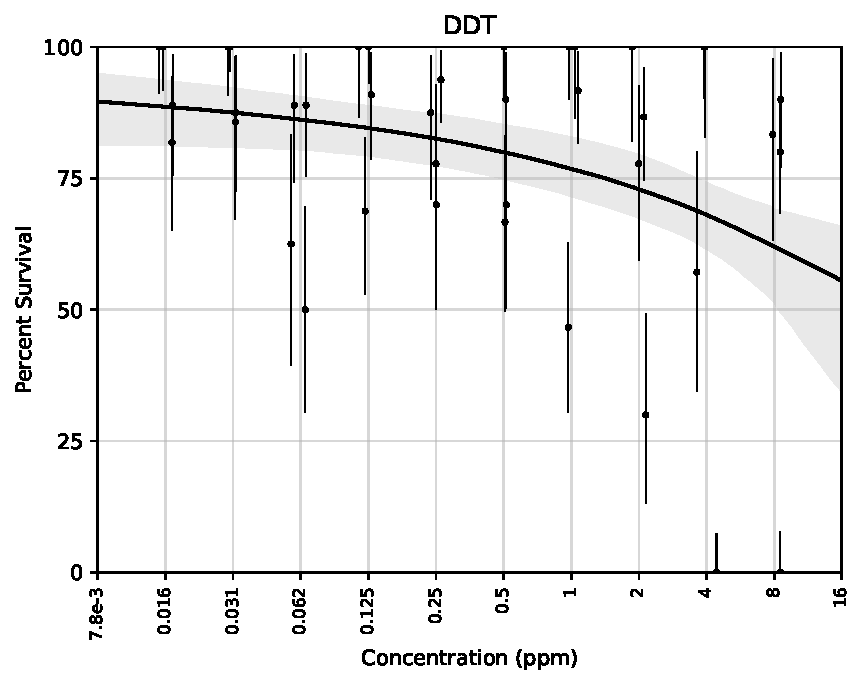
\includegraphics[width = {0.95\textwidth}]{/home/jklimavicz/Documents/merlin_stats_out/images/pdf/DDT.pdf}
      \vspace{-0.05cm}
      \caption*{\textbf{DDT} LC$_{50}$: 37.5 ppm [8.06, 396] \\ 
3 biol. reps; 4 tech. reps; R$^2$: 0.121}
      \vspace{0.1cm}
   \end{subfigure}%
   \begin{subfigure}{0.500\textwidth}
      \centering
      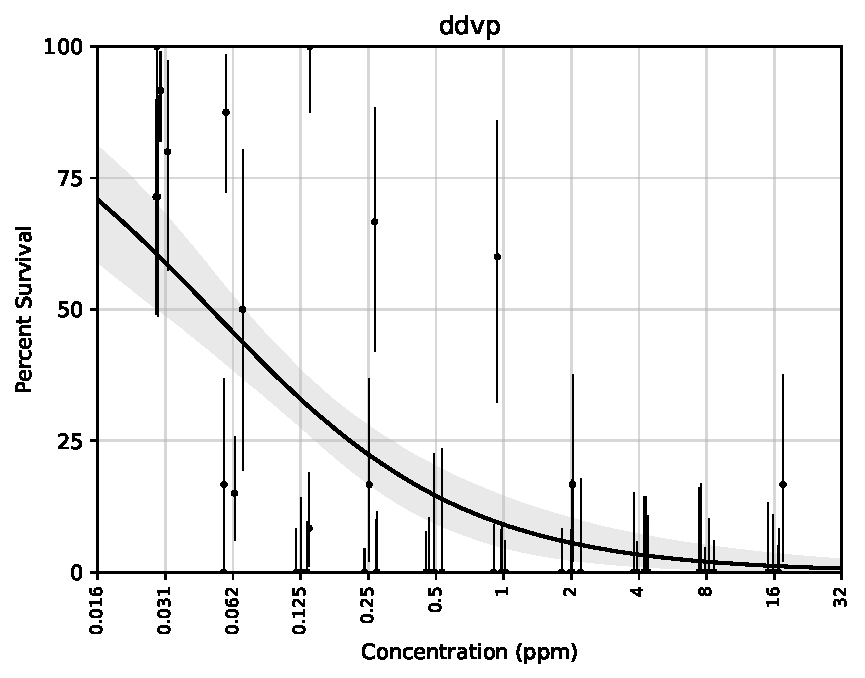
\includegraphics[width = {0.95\textwidth}]{/home/jklimavicz/Documents/merlin_stats_out/images/pdf/ddvp.pdf}
      \vspace{-0.05cm}
      \caption*{\textbf{DDVP} LC$_{50}$: 0.0497 ppm [0.0314, 0.0722] \\ 
4 biol. reps; 5 tech. reps; R$^2$: 0.484}
      \vspace{0.1cm}
   \end{subfigure}%
\vspace{-0.1cm}
   \begin{subfigure}{0.500\textwidth}
      \centering
      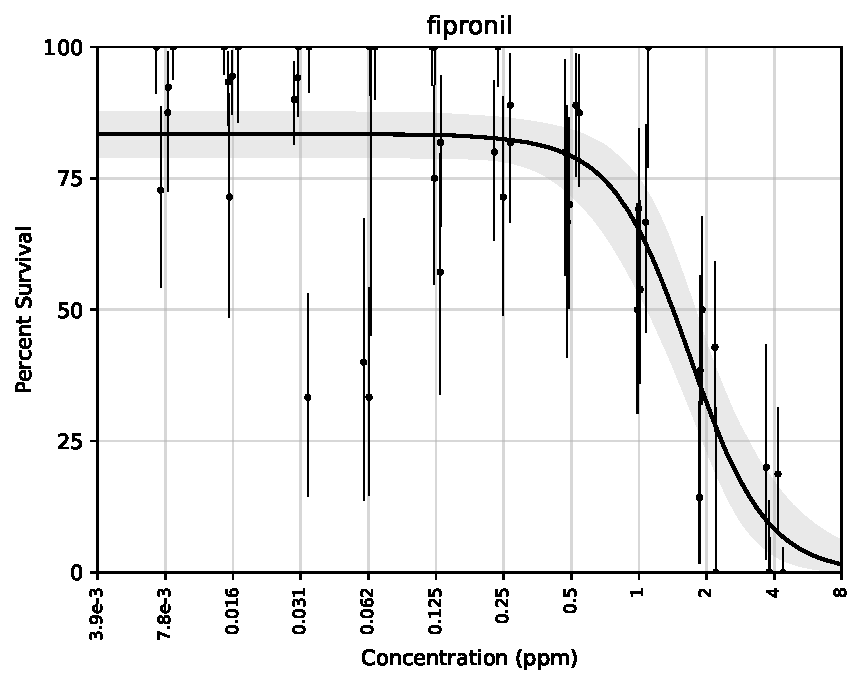
\includegraphics[width = {0.95\textwidth}]{/home/jklimavicz/Documents/merlin_stats_out/images/pdf/fipronil.pdf}
      \vspace{-0.05cm}
      \caption*{\textbf{Fipronil} LC$_{50}$: 1.66 ppm [1.35, 2.1] \\ 
4 biol. reps; 5 tech. reps; R$^2$: 0.68}
      \vspace{0.1cm}
   \end{subfigure}%
   \begin{subfigure}{0.500\textwidth}
      \centering
      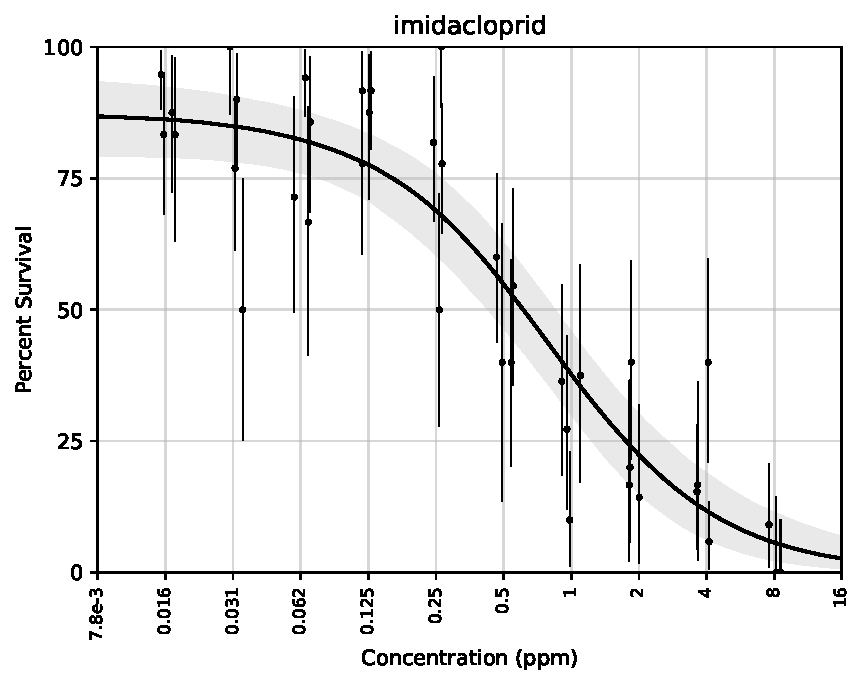
\includegraphics[width = {0.95\textwidth}]{/home/jklimavicz/Documents/merlin_stats_out/images/pdf/imidacloprid.pdf}
      \vspace{-0.05cm}
      \caption*{\textbf{Imidacloprid} LC$_{50}$: 0.789 ppm [0.521, 1.15] \\ 
3 biol. reps; 4 tech. reps; R$^2$: 0.841}
      \vspace{0.1cm}
   \end{subfigure}%
\vspace{-0.1cm}
   \begin{subfigure}{0.500\textwidth}
      \centering
      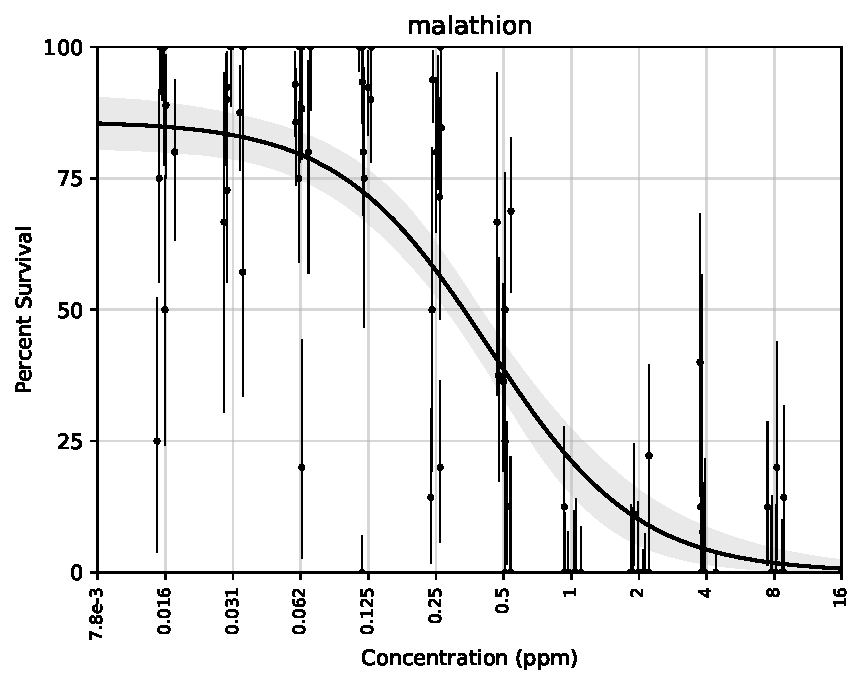
\includegraphics[width = {0.95\textwidth}]{/home/jklimavicz/Documents/merlin_stats_out/images/pdf/malathion.pdf}
      \vspace{-0.05cm}
      \caption*{\textbf{Malathion} LC$_{50}$: 0.426 ppm [0.354, 0.511] \\ 
5 biol. reps; 9 tech. reps; R$^2$: 0.717}
      \vspace{0.1cm}
   \end{subfigure}%
   \begin{subfigure}{0.500\textwidth}
      \centering
      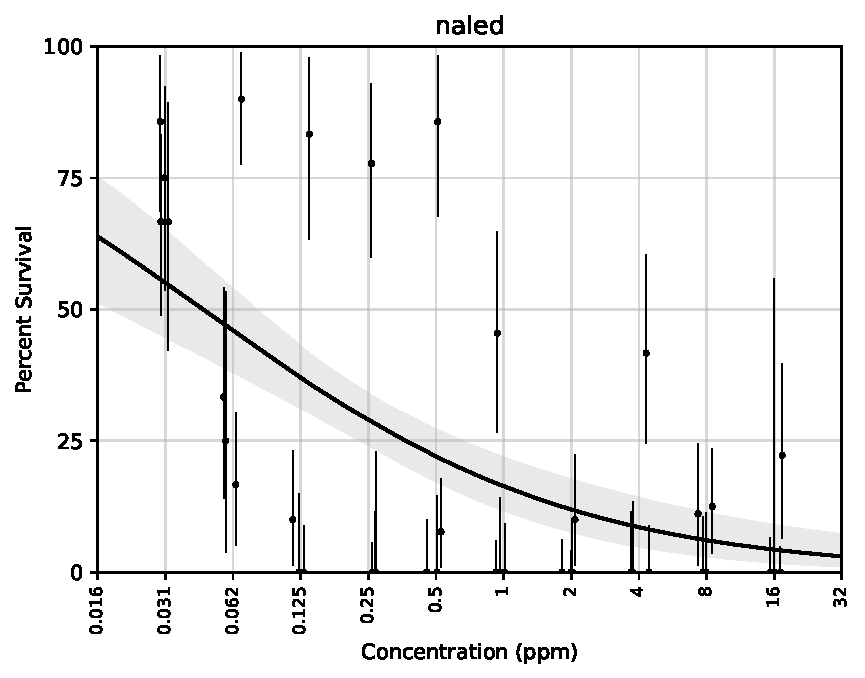
\includegraphics[width = {0.95\textwidth}]{/home/jklimavicz/Documents/merlin_stats_out/images/pdf/naled.pdf}
      \vspace{-0.05cm}
      \caption*{\textbf{Naled} LC$_{50}$: 0.0458 ppm [0.0205, 0.0867] \\ 
3 biol. reps; 4 tech. reps; R$^2$: 0.357}
      \vspace{0.1cm}
   \end{subfigure}%
\end{figure}
\clearpage
\pagebreak
\vspace{-0.1cm}
\begin{figure}[thp!]
   \begin{subfigure}{0.500\textwidth}
      \centering
      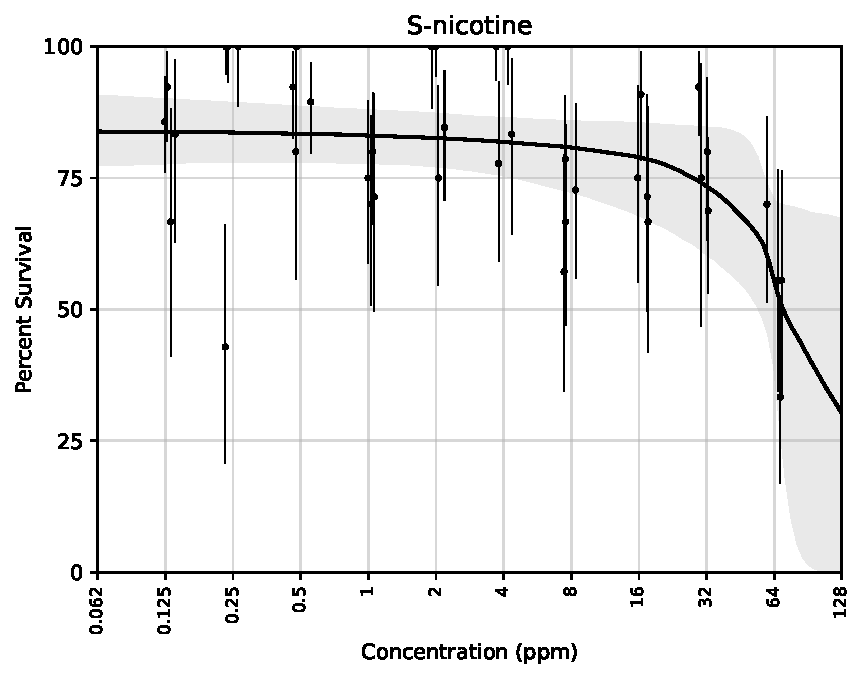
\includegraphics[width = {0.95\textwidth}]{/home/jklimavicz/Documents/merlin_stats_out/images/pdf/S-nicotine.pdf}
      \vspace{-0.05cm}
      \caption*{\textbf{\textit{S}-nicotine} LC$_{50}$: 85.5 ppm [47.3, 1.66e3] \\ 
3 biol. reps; 4 tech. reps; R$^2$: 0.295}
      \vspace{0.1cm}
   \end{subfigure}%
   \begin{subfigure}{0.500\textwidth}
      \centering
      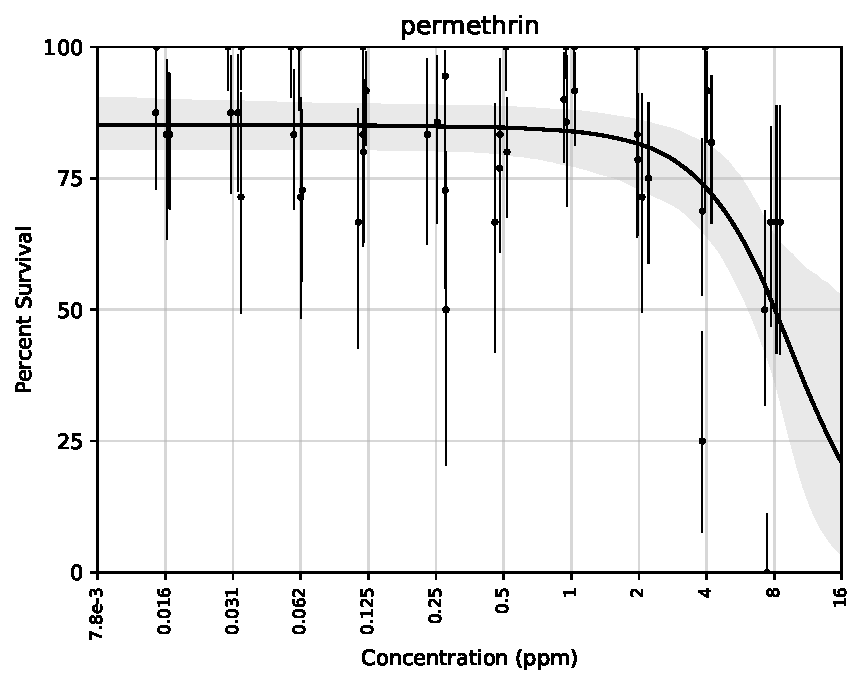
\includegraphics[width = {0.95\textwidth}]{/home/jklimavicz/Documents/merlin_stats_out/images/pdf/permethrin.pdf}
      \vspace{-0.05cm}
      \caption*{\textbf{Permethrin} LC$_{50}$: 9.46 ppm [6.59, 17.8] \\ 
4 biol. reps; 5 tech. reps; R$^2$: 0.317}
      \vspace{0.1cm}
   \end{subfigure}%
\vspace{-0.1cm}
   \begin{subfigure}{0.500\textwidth}
      \centering
      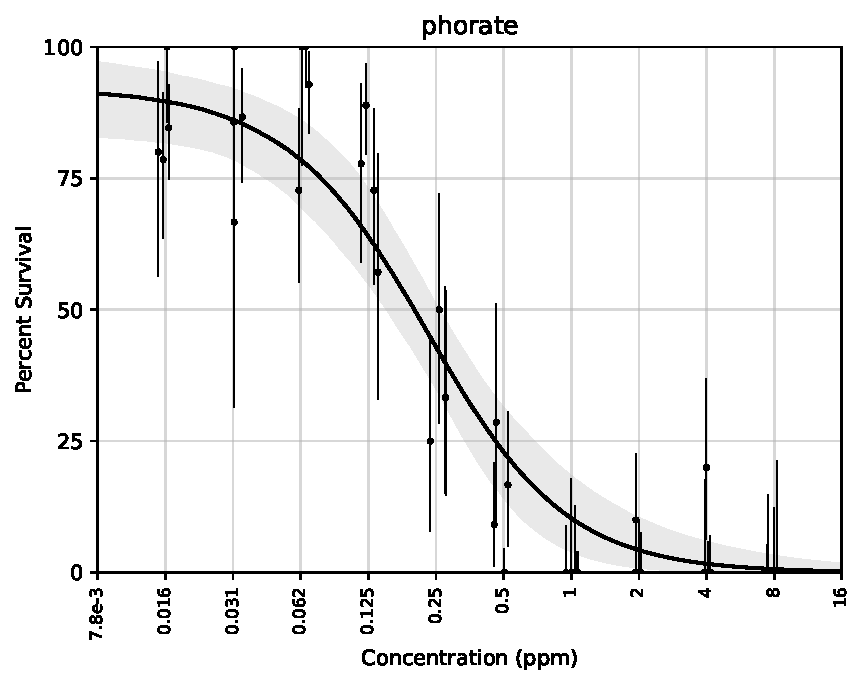
\includegraphics[width = {0.95\textwidth}]{/home/jklimavicz/Documents/merlin_stats_out/images/pdf/phorate.pdf}
      \vspace{-0.05cm}
      \caption*{\textbf{Phorate} LC$_{50}$: 0.226 ppm [0.168, 0.306] \\ 
3 biol. reps; 4 tech. reps; R$^2$: 0.914}
      \vspace{0.1cm}
   \end{subfigure}%
   \begin{subfigure}{0.500\textwidth}
      \centering
      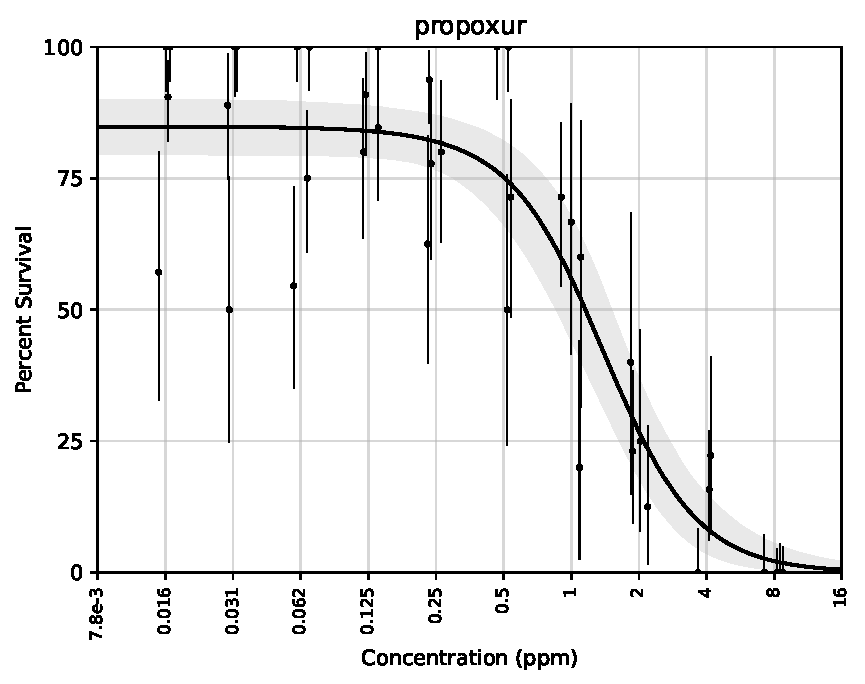
\includegraphics[width = {0.95\textwidth}]{/home/jklimavicz/Documents/merlin_stats_out/images/pdf/propoxur.pdf}
      \vspace{-0.05cm}
      \caption*{\textbf{Propoxur} LC$_{50}$: 1.38 ppm [1.03, 1.8] \\ 
3 biol. reps; 4 tech. reps; R$^2$: 0.817}
      \vspace{0.1cm}
   \end{subfigure}%
\vspace{-0.1cm}
   \begin{subfigure}{0.500\textwidth}
      \centering
      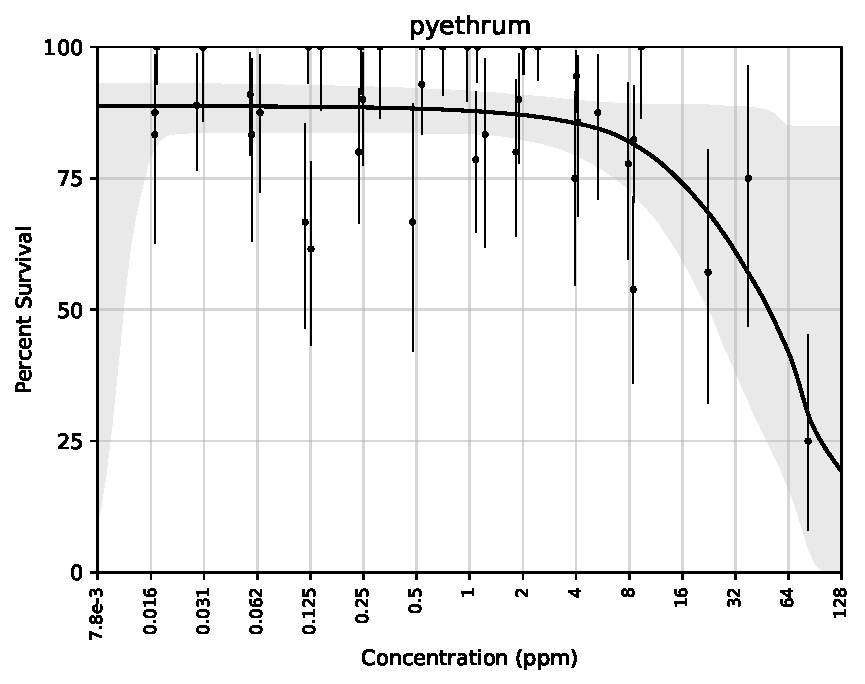
\includegraphics[width = {0.95\textwidth}]{/home/jklimavicz/Documents/merlin_stats_out/images/pdf/pyethrum.pdf}
      \vspace{-0.05cm}
      \caption*{\textbf{Pyethrum} LC$_{50}$: 56.3 ppm [17.2, 369] \\ 
3 biol. reps; 4 tech. reps; R$^2$: 0.435}
      \vspace{0.1cm}
   \end{subfigure}%
\end{figure}
\pagebreak





\end{document}